\documentclass[russian,table]{article}
\usepackage[table]{xcolor}
\usepackage[T1]{fontenc}
\usepackage[utf8]{inputenc}
\usepackage{geometry}
\geometry{verbose,tmargin=2cm,bmargin=2cm,lmargin=1cm,rmargin=1cm}
\usepackage{amsmath}
\usepackage{float}
\usepackage{tikz}
\usetikzlibrary{automata,positioning}
\usepackage{textcomp}
\usepackage{amssymb}
\usepackage{graphicx}
\usepackage{babel}
\usepackage{mathtools}
\usepackage{color}
\usepackage[T2A]{fontenc}
\usepackage{listings}
\usepackage{slashbox}
\usepackage{multirow}
\makeatletter
\@ifundefined{date}{}{\date{}}
\begin{document}

\title{Формальные грамматики. HW\#2}
\author{Тураев Тимур, SPbAU, SE, 604 group}
\maketitle

\paragraph*{1.}

\textit{Постоить обыкновенную грамматику в нормальном виде Хомского для языка Дика $D=\{\varepsilon, ab, aabb, abab, aaabbb, \ldots\}$ над алфавитом $\{a,b\}$. Для этой грамматики и для входной строки $w=abaabba \notin D$, построить таблицу разбора $T_{i,j}$, как в алгоритме Кокка–Касами–Янгера.}

Обыкновенная грамматика не в нормальной форме:
\begin{align*}
S \to aSb \mid SS \mid \varepsilon
\end{align*}

Приведем эту грамматику к нормальной форме Хомского:

\begin{itemize}
\item Удалим длинное правило $S \to aSb$
\begin{align*}
S & \to Tb \mid SS \mid \varepsilon \\
T & \to aS
\end{align*}

\item Удалим $\varepsilon$-правила:
\begin{align*}
S & \to C \mid \varepsilon \\
C & \to Tb \mid CC \\
T & \to a \mid aC
\end{align*}

\item Удалим цепные правила:
\begin{align*}
S & \to Tb \mid CC \mid \varepsilon \\
C & \to Tb \mid CC \\
T & \to a \mid aC
\end{align*}

\item Последний шаг: заменим терминалы на нетерминалы (бесполезных символов в грамматике нет):
\begin{align*}
S & \to TB \mid CC \mid \varepsilon \\
C & \to TB \mid CC \\
T & \to a \mid AC \\
A & \to a \\
B & \to b
\end{align*}
\end{itemize}

Таблица разбора в алгоритме Кокка–Касами–Янгера:

\begin{align*}
\begin{tabular}{c | c c c c c c c}
	~ & a & b & a & a & b & b & a \\
	\hline
	a & \{A, T\} & \{S, C\} & $\varnothing$ & $\varnothing$ & $\varnothing$ & \{S, C\} & $\varnothing$  \\
	b & ~ & \{B\} & $\varnothing$ & $\varnothing$ & $\varnothing$ & $\varnothing$ & $\varnothing$  \\
	a & ~ & ~ & \{A, T\} & $\varnothing$ & \{T\} &  \{S, C\} & $\varnothing$ \\
	a & ~ & ~ & ~ & \{A, T\} &  \{S, C\} & $\varnothing$ & $\varnothing$  \\
	b & ~ & ~ & ~ & ~ & \{B\} & $\varnothing$ & $\varnothing$  \\
	b & ~ & ~ & ~ & ~ & ~ & \{B\} & $\varnothing$  \\
	a & ~ & ~ & ~ & ~ & ~ & ~ & \{A, T\}  \\
\end{tabular}
\end{align*}

По значению отсутствию нетерминала $S$ в $T_{0, 7}$ видно что да, данная строка не принадлежит языку.

\pagebreak

\paragraph*{2.}

\textit{Рассмотреть работу алгоритма Валианта для грамматики, построенной в прошлом упражнении. Среди всех действий, производимых алгоритмом, найти то произведение булевых матриц, после вычисления которого станет верным условие $S \in f(P_{0,6})$, где $S$ — начальный символ грамматики. Описать, когда и как именно вычисляется это произведение — то есть, какая процедура, вызванная с какими значениями, и какой оператор в ней умножает какие две булевы матрицы какого размера, каков результат умножения, и какие элементы $P_{i,j}$ будут этим затронуты?}

% Please add the followin\backslashbox{}{} required packages to your document preamble:
% \usepackage[table,xcdraw]{xcolor}
% If you use beamer only pass "xcolor=table" option, i.e. \documentclass[xcolor=table]{beamer}
\begin{table}[h]
\centering
\begin{tabular}{c|cccccccc}
 &  & a & b & a & a & b & b & a \\ \hline
a & \cellcolor[HTML]{00FF00}\backslashbox{}{} & \cellcolor[HTML]{00FF00} & \cellcolor[HTML]{009901} & \cellcolor[HTML]{009901} & \cellcolor[HTML]{FD6864} & \cellcolor[HTML]{FD6864} & \cellcolor[HTML]{FD6864} & \cellcolor[HTML]{FD6864} \\
b &  & \cellcolor[HTML]{00FF00}\backslashbox{}{} & \cellcolor[HTML]{009901} & \cellcolor[HTML]{009901} & \cellcolor[HTML]{FD6864} & \cellcolor[HTML]{FD6864} & \cellcolor[HTML]{FD6864} & \cellcolor[HTML]{FD6864} \\
a &  &  & \cellcolor[HTML]{00FF00}\backslashbox{}{} & \cellcolor[HTML]{00FF00} & \cellcolor[HTML]{FD6864} & \cellcolor[HTML]{FD6864} & \cellcolor[HTML]{FD6864} & \cellcolor[HTML]{FD6864} \\
a &  &  &  & \cellcolor[HTML]{00FF00}\backslashbox{}{} & \cellcolor[HTML]{FD6864} & \cellcolor[HTML]{FD6864} & \cellcolor[HTML]{FD6864} & \cellcolor[HTML]{FD6864} \\
b &  &  &  &  & \cellcolor[HTML]{00FF00}\backslashbox{}{} & \cellcolor[HTML]{00FF00} & \cellcolor[HTML]{009901} & \cellcolor[HTML]{009901} \\
b &  &  &  &  &  & \cellcolor[HTML]{00FF00}\backslashbox{}{} & \cellcolor[HTML]{009901} & \cellcolor[HTML]{009901} \\
a &  &  &  &  &  &  & \cellcolor[HTML]{00FF00}\backslashbox{}{} & \cellcolor[HTML]{00FF00} \\
 &  &  &  &  &  &  &  & \cellcolor[HTML]{00FF00}\backslashbox{}{}
\end{tabular}
\end{table}

Рассмотрим работу алгоритма Валианта. Единственной функцией, вызванной из $main()$, будет $compute(0, 8)$. Она вызовет $compute(0, 4)$ и $compute(4, 8)$ на двух больших зеленых треугольниках. Эти две функции, в свою очередь, запустят $compute(0, 2)$, $compute(2, 4)$, $compute(4, 6)$, $compute(6, 8)$, который обещают посчитать маленькие светло-зеленые треугольники; и успешно их обсчитают: каждая такая функция $compute(k, k+2)$ запустит единственную $complete(k, k+1, k+1, k+2)$, которая, выполнив 19-я строку алгоритма, заполнит все $T_{i, j}$, стоящие на светло-зеленых клетках. Получится следующее:

% Please add the following required packages to your document preamble:
% \usepackage[table,xcdraw]{xcolor}
% If you use beamer only pass "xcolor=table" option, i.e. \documentclass[xcolor=table]{beamer}
\begin{table}[h]
\centering
\begin{tabular}{c|cccccccc}
 &  & a & b & a & a & b & b & a \\ \hline
a & \cellcolor[HTML]{00FF00}-- & \cellcolor[HTML]{00FF00}\{A, T\} & \cellcolor[HTML]{009901} & \cellcolor[HTML]{009901} & \cellcolor[HTML]{FD6864} & \cellcolor[HTML]{FD6864} & \cellcolor[HTML]{FD6864} & \cellcolor[HTML]{FD6864} \\
b &  & \cellcolor[HTML]{00FF00}-- & \cellcolor[HTML]{009901} & \cellcolor[HTML]{009901} & \cellcolor[HTML]{FD6864} & \cellcolor[HTML]{FD6864} & \cellcolor[HTML]{FD6864} & \cellcolor[HTML]{FD6864} \\
a &  &  & \cellcolor[HTML]{00FF00}-- & \cellcolor[HTML]{00FF00}\{A, T\} & \cellcolor[HTML]{FD6864} & \cellcolor[HTML]{FD6864} & \cellcolor[HTML]{FD6864} & \cellcolor[HTML]{FD6864} \\
a &  &  &  & \cellcolor[HTML]{00FF00}-- & \cellcolor[HTML]{FD6864} & \cellcolor[HTML]{FD6864} & \cellcolor[HTML]{FD6864} & \cellcolor[HTML]{FD6864} \\
b &  &  &  &  & \cellcolor[HTML]{00FF00}-- & \cellcolor[HTML]{00FF00}\{B\} & \cellcolor[HTML]{009901} & \cellcolor[HTML]{009901} \\
b &  &  &  &  &  & \cellcolor[HTML]{00FF00}-- & \cellcolor[HTML]{009901} & \cellcolor[HTML]{009901} \\
a &  &  &  &  &  &  & \cellcolor[HTML]{00FF00}-- & \cellcolor[HTML]{00FF00}\{A, T\} \\
 &  &  &  &  &  &  &  & \cellcolor[HTML]{00FF00}--
\end{tabular}
\end{table}

Кроме обсчета маленьких светло-зеленых треугольников, функии $compute(0, 4)$ и $compute(4, 8)$ обсчитают и темно-зеленые квадраты:

% Please add the following required packages to your document preamble:
% \usepackage[table,xcdraw]{xcolor}
% If you use beamer only pass "xcolor=table" option, i.e. \documentclass[xcolor=table]{beamer}
\begin{table}[h]
\centering
\begin{tabular}{c|cccccccc}
 &  & a & b & a & a & b & b & a \\ \hline
a & \cellcolor[HTML]{00FF00}-- & \cellcolor[HTML]{00FF00}\{A, T\} & \cellcolor[HTML]{009901}\{S, C\} & \cellcolor[HTML]{009901}$\varnothing$ & \cellcolor[HTML]{FD6864} & \cellcolor[HTML]{FD6864} & \cellcolor[HTML]{FD6864} & \cellcolor[HTML]{FD6864} \\
b &  & \cellcolor[HTML]{00FF00}-- & \cellcolor[HTML]{009901}\{B\} & \cellcolor[HTML]{009901}$\varnothing$ & \cellcolor[HTML]{FD6864} & \cellcolor[HTML]{FD6864} & \cellcolor[HTML]{FD6864} & \cellcolor[HTML]{FD6864} \\
a &  &  & \cellcolor[HTML]{00FF00}-- & \cellcolor[HTML]{00FF00}\{A, T\} & \cellcolor[HTML]{FD6864} & \cellcolor[HTML]{FD6864} & \cellcolor[HTML]{FD6864} & \cellcolor[HTML]{FD6864} \\
a &  &  &  & \cellcolor[HTML]{00FF00}-- & \cellcolor[HTML]{FD6864} & \cellcolor[HTML]{FD6864} & \cellcolor[HTML]{FD6864} & \cellcolor[HTML]{FD6864} \\
b &  &  &  &  & \cellcolor[HTML]{00FF00}-- & \cellcolor[HTML]{00FF00}\{B\} & \cellcolor[HTML]{009901}$\varnothing$ & \cellcolor[HTML]{009901}$\varnothing$ \\
b &  &  &  &  &  & \cellcolor[HTML]{00FF00}-- & \cellcolor[HTML]{009901}\{B\} & \cellcolor[HTML]{009901}$\varnothing$ \\
a &  &  &  &  &  &  & \cellcolor[HTML]{00FF00}-- & \cellcolor[HTML]{00FF00}\{A, T\} \\
 &  &  &  &  &  &  &  & \cellcolor[HTML]{00FF00}--
\end{tabular}
\end{table}

Таким образом, функции $compute(0, 4)$ и $compute(4, 8)$ (внутри вызова $compute(0, 8)$) закончат свою работу. Далее вызовется функция $\textbf{complete(0, 4, 4, 8)}$.
Она поделит большой красный квадрат на 4 квадрата $D, E, C, D'$ и запустит $complete(C)$, то есть $complete(2,4,4,6)$. Эта функция его обсчитает аналогично тому как обсчитывались темно-зеленые квадраты. 9-я строка алгоритма внутри $\textbf{complete(0, 4, 4, 8)}$ выполнилась.

% Please add the following required packages to your document preamble:
% \usepackage{multirow}
% \usepackage[table,xcdraw]{xcolor}
% If you use beamer only pass "xcolor=table" option, i.e. \documentclass[xcolor=table]{beamer}
\begin{table}[h]
\centering
\begin{tabular}{c|cccccccc}
 &  & a & b & a & a & b & b & a \\ \hline
a & \cellcolor[HTML]{00FF00}-- & \cellcolor[HTML]{00FF00}\{A, T\} & \cellcolor[HTML]{009901}\{S, C\} & \cellcolor[HTML]{009901}$\varnothing$ & \multicolumn{2}{c}{\cellcolor[HTML]{FD6864}} & \multicolumn{2}{c}{\cellcolor[HTML]{FD6864}} \\
b &  & \cellcolor[HTML]{00FF00}-- & \cellcolor[HTML]{009901}\{B\} & \cellcolor[HTML]{009901}$\varnothing$ & \multicolumn{2}{c}{\multirow{-2}{*}{\cellcolor[HTML]{FD6864}D}} & \multicolumn{2}{c}{\multirow{-2}{*}{\cellcolor[HTML]{FD6864}E}} \\
a &  &  & \cellcolor[HTML]{00FF00}-- & \cellcolor[HTML]{00FF00}\{A, T\} & \cellcolor[HTML]{FD6864}$\varnothing$ & \cellcolor[HTML]{FD6864}\{T\} & \multicolumn{2}{c}{\cellcolor[HTML]{FD6864}} \\
a &  &  &  & \cellcolor[HTML]{00FF00}-- & \cellcolor[HTML]{FD6864}\{A, T\} & \cellcolor[HTML]{FD6864}\{S, C\} & \multicolumn{2}{c}{\multirow{-2}{*}{\cellcolor[HTML]{FD6864}D'}} \\
b &  &  &  &  & \cellcolor[HTML]{00FF00}-- & \cellcolor[HTML]{00FF00}\{B\} & \cellcolor[HTML]{009901}$\varnothing$ & \cellcolor[HTML]{009901}$\varnothing$ \\
b &  &  &  &  &  & \cellcolor[HTML]{00FF00}-- & \cellcolor[HTML]{009901}\{B\} & \cellcolor[HTML]{009901}$\varnothing$ \\
a &  &  &  &  &  &  & \cellcolor[HTML]{00FF00}-- & \cellcolor[HTML]{00FF00}\{A, T\} \\
 &  &  &  &  &  &  &  & \cellcolor[HTML]{00FF00}--
\end{tabular}
\end{table}

Далее выполнятся строки 10-11 (обсчет матрицы $D$) и стркои 12-13 (обсчет матрицы $D'$) внутри $\textbf{complete(0, 4, 4, 8)}$.

\begin{table}[h]
\centering
\begin{tabular}{c|cccccccc}
 &  & a & b & a & a & b & b & a \\ \hline
a & \cellcolor[HTML]{00FF00}-- & \cellcolor[HTML]{00FF00}\{A, T\} & \cellcolor[HTML]{009901}\{S, C\} & \cellcolor[HTML]{009901}$\varnothing$ & \cellcolor[HTML]{FD6864}$\varnothing$ & \cellcolor[HTML]{FD6864}$\varnothing$ & \multicolumn{2}{c}{\cellcolor[HTML]{FD6864}} \\
b &  & \cellcolor[HTML]{00FF00}-- & \cellcolor[HTML]{009901}\{B\} & \cellcolor[HTML]{009901}$\varnothing$ & \cellcolor[HTML]{FD6864}$\varnothing$ & \cellcolor[HTML]{FD6864}$\varnothing$ & \multicolumn{2}{c}{\multirow{-2}{*}{\cellcolor[HTML]{FD6864}E}} \\
a &  &  & \cellcolor[HTML]{00FF00}-- & \cellcolor[HTML]{00FF00}\{A, T\} & \cellcolor[HTML]{FD6864}$\varnothing$ & \cellcolor[HTML]{FD6864}\{T\} & \cellcolor[HTML]{CB0000}\{S, C\} & \cellcolor[HTML]{CB0000}$\varnothing$ \\
a &  &  &  & \cellcolor[HTML]{00FF00}-- & \cellcolor[HTML]{FD6864}\{A, T\} & \cellcolor[HTML]{FD6864}\{S, C\} & \cellcolor[HTML]{CB0000}$\varnothing$ & \cellcolor[HTML]{CB0000}$\varnothing$ \\
b &  &  &  &  & \cellcolor[HTML]{00FF00}-- & \cellcolor[HTML]{00FF00}\{B\} & \cellcolor[HTML]{009901}$\varnothing$ & \cellcolor[HTML]{009901}$\varnothing$ \\
b &  &  &  &  &  & \cellcolor[HTML]{00FF00}-- & \cellcolor[HTML]{009901}\{B\} & \cellcolor[HTML]{009901}$\varnothing$ \\
a &  &  &  &  &  &  & \cellcolor[HTML]{00FF00}-- & \cellcolor[HTML]{00FF00}\{A, T\} \\
 &  &  &  &  &  &  &  & \cellcolor[HTML]{00FF00}--
\end{tabular}
\end{table}

Наконец алгоритм перейдет к строке \textbf{14}: $P_E = P_E \cup (T_B \times T_{D'})$. Подматрица $P_E$ это матрица $\bigl(\begin{smallmatrix} P_{0, 6} & P_{0, 7} \\ P_{1, 6} &P_{1, 7} \end{smallmatrix} \bigr)$. Подматрица $T_B$ на рисунке выше -- это первая темно-зеленая, то есть $\bigl(\begin{smallmatrix} P_{0, 2} & P_{0, 3} \\ P_{1, 2} &P_{1, 3} \end{smallmatrix} \bigr) = \bigl(\begin{smallmatrix} \{S, C\} & \varnothing \\ \{B\} & \varnothing \end{smallmatrix} \bigr)$, а матрица $T_D'$ это темно-красная матрица $\bigl(\begin{smallmatrix} P_{2, 6} & P_{2, 7} \\ P_{3, 6} &P_{3, 7} \end{smallmatrix} \bigr)  = \bigl(\begin{smallmatrix} \{S, C\} & \varnothing \\ \varnothing & \varnothing \end{smallmatrix} \bigr)$. Именно их алгоритм собираться перемножать, используя произведение булевых матриц.

Алгоритм работает так: по каждой паре нетерминалов $\{A, B\}$ (их у нас $|N|^2 = 25$) строются две булевы матрицы: матрица $X^A$, элемент которой (булев бит) означает есть ли нетерминал $A$ в соответствующем элементе первой матрицы; и матрица $Y^B$, элемент которой (булев бит) означает есть ли нетерминал $B$ в соответствующем элементе второй матрицы. Получившаяся в результате умножения булева матрица, которую можно назвать $Z^{AB}$, означает <<где в итоговой матрице $(T_B \times T_{D'})$ будет элемент-пара нетерминалов $\{A, B\}$>>. 

В нашем случае, когда дело дойдет до рассмотрения пары $\mathbf{\{C, C\}}$, матрица $X^C$ будет иметь вид $\bigl(\begin{smallmatrix} 1&0\\0&0 \end{smallmatrix} \bigr)$, а матрица $Y^C$ $\bigl(\begin{smallmatrix} 1&0\\0&0 \end{smallmatrix} \bigr)$. Их произведение: $\bigl(\begin{smallmatrix} 1&0\\0&0 \end{smallmatrix} \bigr)$, что означает, пара $\{C, C\}$ гарантированно будет стоять на первой строке первого столбца матрицы $P_E$. А это в свою очередь означает, что когда алгоритм дойдет до 16 строки ($complete(E)$), затем вызовется ($complete(D) = complete(0, 1, 6, 7)$), в матрице T на месте $(0, 6)$ появится нетерминал $S$, потому что существует правило $S \to CC$ (вместе с ним, в этом же множестве нетерминалов, из-за пары $\{C, C\}$ появится еще и $C$, так как существует правило $C \to CC$).

%Среди всех действий, производимых алгоритмом, найти то произведение булевых матриц, после вычисления которого станет верным условие $S \in f(P_{0,6})$, где $S$ — начальный символ грамматики. Описать, когда и как именно вычисляется это произведение — то есть, какая процедура, вызванная с какими значениями, и какой оператор в ней умножает какие две булевы матрицы какого размера, каков результат умножения, и какие элементы $P_{i,j}$ будут этим затронуты?%

Итак, собираем все вместе и отвечаем на вопросы в задании:

\begin{itemize}
\item какая процедура c какими параметрами -- $\mathbf{complete(0, 4, 4, 8)}$ (вызванная из $compute(0, 8)$, которая в свою очередь вызвана из $main()$)
\item какой оператор в ней -- 14-я строка алгоритма, $\mathbf{(T_B \times T_{D'})}$
\item какие две булевы матрицы какого размера -- умножаются 2 матрицы $2 \times 2$: $\mathbf{X^C = \bigl(\begin{smallmatrix} 1&0\\0&0 \end{smallmatrix} \bigr)}$ и $\mathbf{Y^C = \bigl(\begin{smallmatrix} 1&0\\0&0 \end{smallmatrix} \bigr)}$
\item каков результат умножения этих булевых матриц -- $\mathbf{Z^{CC} = \bigl(\begin{smallmatrix} 1&0\\0&0 \end{smallmatrix} \bigr)}$
\item общий результат умножения $(T_B \times T_{D'})$ -- $\mathbf{\bigl(\begin{smallmatrix} \{\{S, S\}, \{C, C\}, \{S, C\}, \{C, S\}\} & \varnothing  \\ \{\{B, S\}, \{B, C\} & \varnothing \end{smallmatrix} \bigr)}$
\item какие элементы $P_{i,j}$ будут этим затронуты -- при этом умножении затронуты будут элементы подматрицы $P_E = \bigl(\begin{smallmatrix} P_{0, 6} & P_{0, 7} \\ P_{1, 6} &P_{1, 7} \end{smallmatrix} \bigr)$
\end{itemize}

\pagebreak

\paragraph*{3.}

\textit{Замкнут ли класс LL языков относительно пересечения с регулярными языками? Если замкнут, привести построение, а если незамкнут, привести пример LL грамматики и регулярного языка с доказательством несуществования LL грамматики для их пересечения}

Рассмотрим язык $L_1$, который задает все строки четной длины, первая половина которых состоит только из букв a, а вторая -- из любых сочетаний букв b и c:

\begin{align*}
L_1 = \{ a^n(b|c)^n \mid n \geqslant 0 \}
\end{align*}

Это $LL(1)$-язык, для него можно построить такую грамматику:

\begin{align*}
S & \to aSB \mid \varepsilon \\
B & \to b \mid c 
\end{align*}

и следующую таблицу разбора:

\begin{align*}
\begin{tabular}{c | c c c c |}
	~ & a & b & c & $\varepsilon$ \\
	\hline
	S & S $\to$ aSB & S $\to$ $\varepsilon$ & S $\to$ $\varepsilon$ & S $\to$ $\varepsilon$ \\
	B & -- & B $\to$ b & B $\to$ c& B $\to$ $\varepsilon$ \\
	\hline
\end{tabular}
\end{align*}

Наряду с $L_1$ рассмотрим язык $L_2$, задающий все слова, в котором сначала идет какое-то (возможно нулевое) число букв a, а затем какое-то (возможно нулевое) число букв b:

\begin{align*}
L_2 = \{ a^nb^m + a^nc^m\mid n,m \geqslant 0 \}
\end{align*}

Это тоже $LL(1)$-язык, для него можно построить такую грамматику:

\begin{align*}
S & \to AE \\
A & \to aA \mid \varepsilon \\ 
E & \to bB \mid cC \mid \varepsilon  \\
B & \to bB \mid \varepsilon \\
C & \to cC \mid \varepsilon
\end{align*}

и следующую таблицу разбора:

\begin{align*}
\begin{tabular}{c | c c c c |}
	~ & a & b & c & $\varepsilon$ \\
	\hline
	S & S $\to$ AE & S $\to$ AE & S $\to$ AE & S $\to$ AE \\
	E & -- & E $\to$ bB & E $\to$ cC & E $\to$ $\varepsilon$ \\
	B & -- & B $\to$ bB & --  & B $\to$ $\varepsilon$ \\
	C & -- & -- & C $\to$ cC & C $\to$ $\varepsilon$ \\
	\hline
\end{tabular}
\end{align*}

Кроме того, этот язык, очевидно, является регулярным:

\begin{align*}
L_2 = a^*(b^* \mid c^*) \\ 
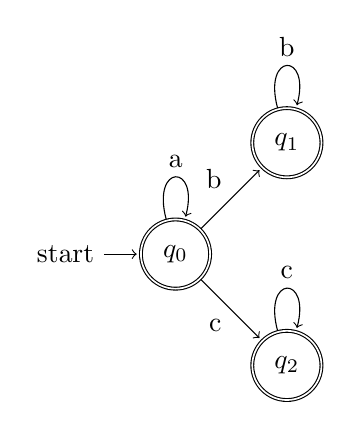
\begin{tikzpicture}[shorten >=1pt,node distance=2cm,on grid,auto] 
   \node[state,initial,accepting] (q_0)   {$q_0$}; 
   \node[state,accepting] (q_1) [above right=of q_0] {$q_1$}; 
   \node[state,accepting] (q_2) [below right=of q_0] {$q_2$};
    \path[->]
    (q_0) edge  node {b} (q_1)
          edge  node [swap] {c} (q_2)
          edge  [loop above] node {a} ()
    (q_1) edge [loop above] node  {b} ()
    (q_2) edge [loop above] node  {c} ();
\end{tikzpicture}
\end{align*}

Пересечением этих языков является язык $L_3$:

\begin{align*}
L_1 \cap L_2 = L_3 = \{ a^nb^n + a^nc^n\mid n \geqslant 0 \}
\end{align*}

который, как мы знаем, не является $LL(k)$ ни для какого $k$ (см пример 8.4 конспекта 11 лекции).

Отсюда делаем вывод, что класс LL языков не замкнут относительно пересечения с регулярными языками.

\end{document}